\tinypar{Summary} Angelo Porrello has been a member of the research group AimageLab at the Department of Engineering "Enzo Ferrari" in Modena for seven years. He currently holds a post-doc position as Research Assistant. He is an active member of the scientific community, with his work particularly focusing on Artificial Intelligence (AI) and Computer Vision. He is the author of more than twenty scientific articles, published through peer review at international conferences and journals (e.g., CVPR, ECCV, ICCV, NeurIPS, etc.). His primary research areas include the continuous training of neural networks and the development of predictive AI systems and video-analytics in the field of video surveillance. In the biennium 2022-2023, he served as a scientific advisor for Cristail, a startup that develops intelligent asset management tools using advanced AI techniques.
%
\subsection{Scholar}
%
Metrics updated on 02/07/2024.
\vspace{-0.8em}
\begin{center}
\begin{tabular}{cc}
     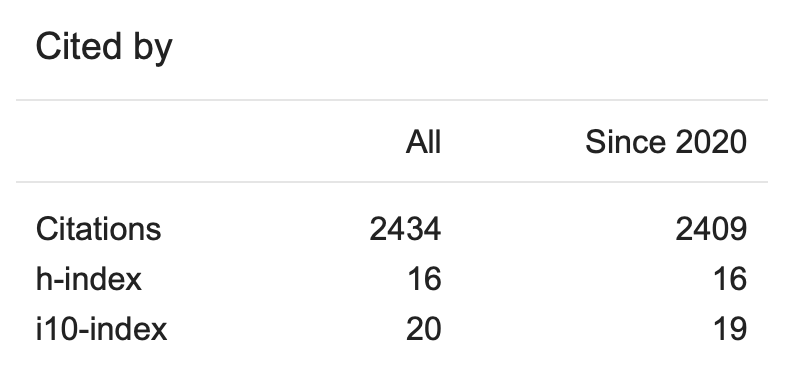
\includegraphics[width=0.55\textwidth]{images/scholar-numbers-eng.png} & 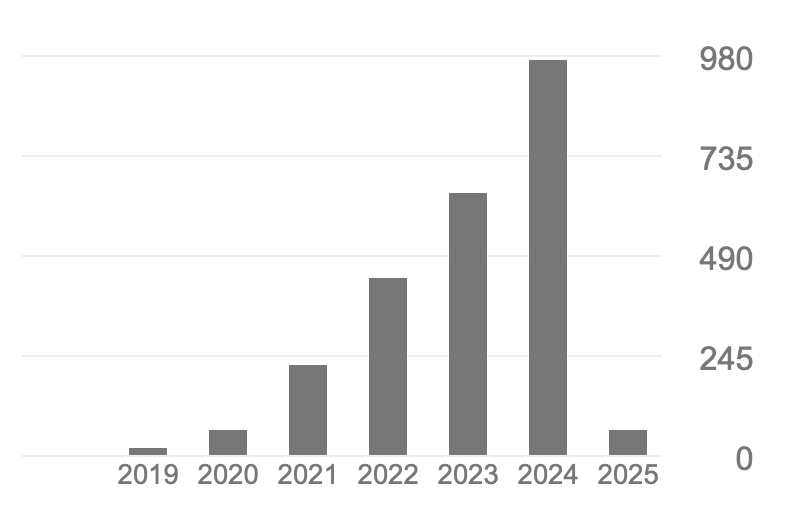
\includegraphics[width=0.4\textwidth]{images/scholar-plot-eng.png}
\end{tabular}    
\end{center}